\chapter{Tinjauan Pustaka dan Dasar Teori}

\section{Tinjauan Pustaka}

Berisi tugas akhir-tugas akhir terdahulu yang terkait dengan judul skripsi yang dilakukan. Hal ini meliputi skripsi, tesis, atau publikasi terdahulu yang terkait dengan judul skripsi yang diusulkan. Lakukan pembahasan secara sistemastis dengan menjelaskan masalah apa yang dilakukan oleh tugas akhir terdahulu, kontribusi yang dilakukan, serta analisis penulis terkait dengan keunggulan dan keterbatasan tugas akhir. 

Setelah membahas berbagai tugas akhir terdahulu, maka alangkah baiknya penulis melakukan rangkuman terutama terkait dengan peluang pengembangan atau tugas akhir yang akan dilakukan.


\section{Dasar Teori}

Berisi teori-teori yang menjadi dasar solusi atau produk hasil skripsi. Dasar teori pada umumnya diperoleh melalui buku referensi, publikasi tugas akhir, dan informasi web yang dapat dipertanggungjawabkan. Hindari penggunaan dasar teori melalui tautan wikipedia, surat kabar, atau portal berita.

\subsection{Pengenalan Aplikasi Permainan}

Proses pembuatan \textit{game} dimulai dari pembuatan \textit{game design document} dimana 
dokumen ini akan menjadi landasan pengembangan game tersebut serta menginformasikan gambaran keseluruhan game yang akan dibuat \cite{ferdiana2012agile}. \textcolor{red}{\textit{Catatan: apapun yang diambil dari tulisan orang lain harus disitasi seperti dicontohkan \cite{ferdiana2012agile}.}}

\begin{figure}[h]
	\centering
	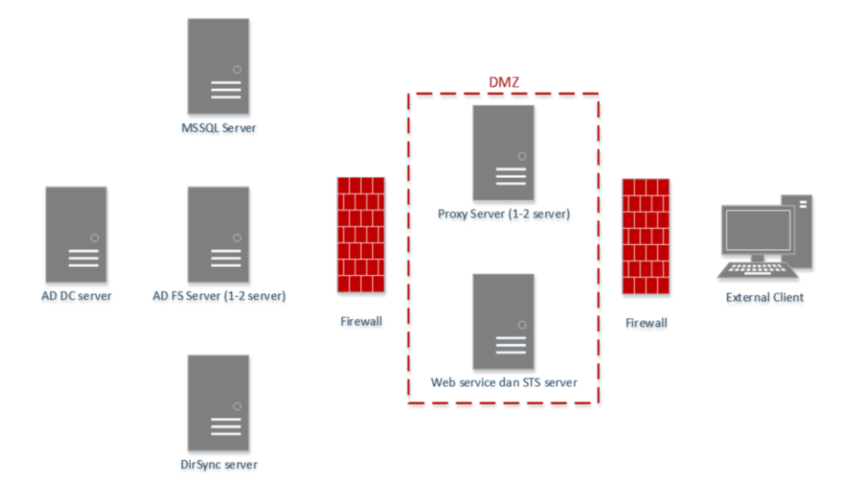
\includegraphics[width=12cm]{contents/chapter-2/gambar-buatan-sendiri.png}
	\caption[Contoh gambar]{Contoh gambar \cite{lukito2016}}
	\label{Fig:gambar-buatan-sendiri}
\end{figure}



\textit{Game design document} adalah sebuah bagian penting dalam pembuatan game baik itu elemen-elemen penyusunnya maupun proses pengembangannya. Game design yang telah dibuat, dijabarkan satu persatu mengenai tahapan dalam pembuatan game dan hasilnya disatukan dalam bentuk dokumentasi \textit{game design document} yang digunakan oleh \textit{developer} sebagai buku petunjuk bagaimana membuat \textit{game} \cite{lukito2016}.

Dalam buku \textit{Game Design Essentials} disebutkan \textit{game design document} merupakan metode yang menghubungkan elemen-elemen penyusun \textit{game}, baik itu \textit{art, sound, program, 
gameplay} sehingga semuanya terdokumentasi menjadi satu dan menjadi acuan bagi para \textit{developer} dalam membuat \textit{game} \cite{wibirama2013dual}. 

\subsection{Dasar Teori Lainnya}

\section{Analisis Perbandingan Metode}

Di dalam tinjauan pustaka hasil akhirnya adalah analisis secara kualitatif atau pun secara kuantitatif kelebihan dan kekurangan metode jika dikaitkan dengan masalah, batasan-batasan masalah dan solusi yang dinginkan. Analisis kuantitatif tidak wajib teapi mempunyai nilai tambah di dalam tugas akhir saudara. Bagian ini menjelaskan kenapa metode tersebut dipilih dan uraikan dengan lebih jelas metode pelaksanaan tugas akhir yang ingin Anda lakukan. 

\section{Pertanyaan Tugas Akhir (Jika Perlu)}

Pertanyaan tugas akhir bersifat opsional dan dapat ditambahkan untuk menekankan hal-hal yang hendak diketahui dari tugas akhir berdasar pada tujuan tugas akhir. Pertanyaan tugas akhir dikenal dengan RQ (\textit{Research Question}) dan harus memiliki keterkaitan dengan RO (\textit{Research Objective}). Satu RO dapat memiliki satu atau lebih dari satu RQ. 

